% arara: lualatex
\pdfoptionpdfminorversion 7
\documentclass{beamer}
\AtBeginSection{\frame{\sectionpage}}

\defbeamertemplate{section page}{mine}[1][]{%
  \begin{centering}
    {\usebeamerfont{section name}\usebeamercolor[fg]{section name}#1}
    \vskip1em\par
    \begin{beamercolorbox}[sep=12pt,center]{part title}
      \usebeamerfont{section title}\insertsection\par
    \end{beamercolorbox}
  \end{centering}
}
\setbeamertemplate{section page}[mine]

\usepackage{pgfplots}

\title{High Pressure Ignition Chemistry of Alternative Fuels}
\author{Bryan W. Weber}
\institute{Prepared for Ph.D. Defense}
\date{June 19, 2014}

\beamertemplatenavigationsymbolsempty

\setbeamertemplate{footline}
{%
\begin{beamercolorbox}[sep=2mm]{}

\includegraphics[height=0.25in]{logo}
\hfill
{\color{gray} \insertpagenumber{}/\insertpresentationendpage}
\end{beamercolorbox}
}%

\graphicspath{ {figures/} }

\begin{document}

\maketitle

\begin{frame}<1-4>[label=economy]{Combustion drives the energy economy}
    \only<2>{
        \begin{center}
            \begin{tikzpicture}
    \begin{axis}[
        xtick={0,1,...,7},
        xticklabels={
            {Petroleum},
            {Natural Gas},
            {Coal},
            {Nuclear},
            {Hydropower},
            {Biomass},
            {Renewable Energy},
            {Other},
        },
        x tick label style={
            text height=2ex,
            rotate=45,
            anchor=north east,
            font=\footnotesize,
            yshift=10pt,
            align=right,
        },
        ybar,
        ylabel={Percent},
        title={United States Energy Consumption by Fuel Source},
        height=0.8\textheight,
        width=\textwidth,
        area legend,
    ]
        \pgfmathsetmacro\totaltwentythirteen{96.49}
        \addplot coordinates {
            (0,35.97/\totaltwentythirteen*100)
            (1,26.22/\totaltwentythirteen*100)
            (2,18.46/\totaltwentythirteen*100)
            (3,7.93/\totaltwentythirteen*100)
            (4,2.59/\totaltwentythirteen*100)
            (5,2.68/\totaltwentythirteen*100)
            (6,2.26/\totaltwentythirteen*100)
            (7,0.39/\totaltwentythirteen*100)
        };
        \pgfmathsetmacro\totaltwentyforty{106.31}
        \addplot coordinates {
            (0,35.35/\totaltwentyforty*100)
            (1,32.32/\totaltwentyforty*100)
            (2,18.75/\totaltwentyforty*100)
            (3,8.49/\totaltwentyforty*100)
            (4,2.90/\totaltwentyforty*100)
            (5,4.26/\totaltwentyforty*100)
            (6,3.89/\totaltwentyforty*100)
            (7,0.35/\totaltwentyforty*100)
        };
        \legend{2013,2040}
        \node[anchor=west,align=left] at (axis cs:3.5,20) {Data from EIA Annual\\Energy Report 2014};
    \end{axis}
\end{tikzpicture}

        \end{center}
    }
    \only<1,3->{
        \begin{itemize}
            \item Combustion is predicted to remain the dominant energy conversion process for many years into the future
            \item The combustion of fossil fuels has been implicated in a number of harmful effects on human health, the environment, and the economy
            \item Two solutions have been proposed:
                \begin{itemize}
                    \item<alert@4> Better engines
                    \item<alert@5> Better fuels
                \end{itemize}
        \end{itemize}
    }
\end{frame}

\begin{frame}{Better engines have higher efficiency and lower emissions}
    \begin{center}
        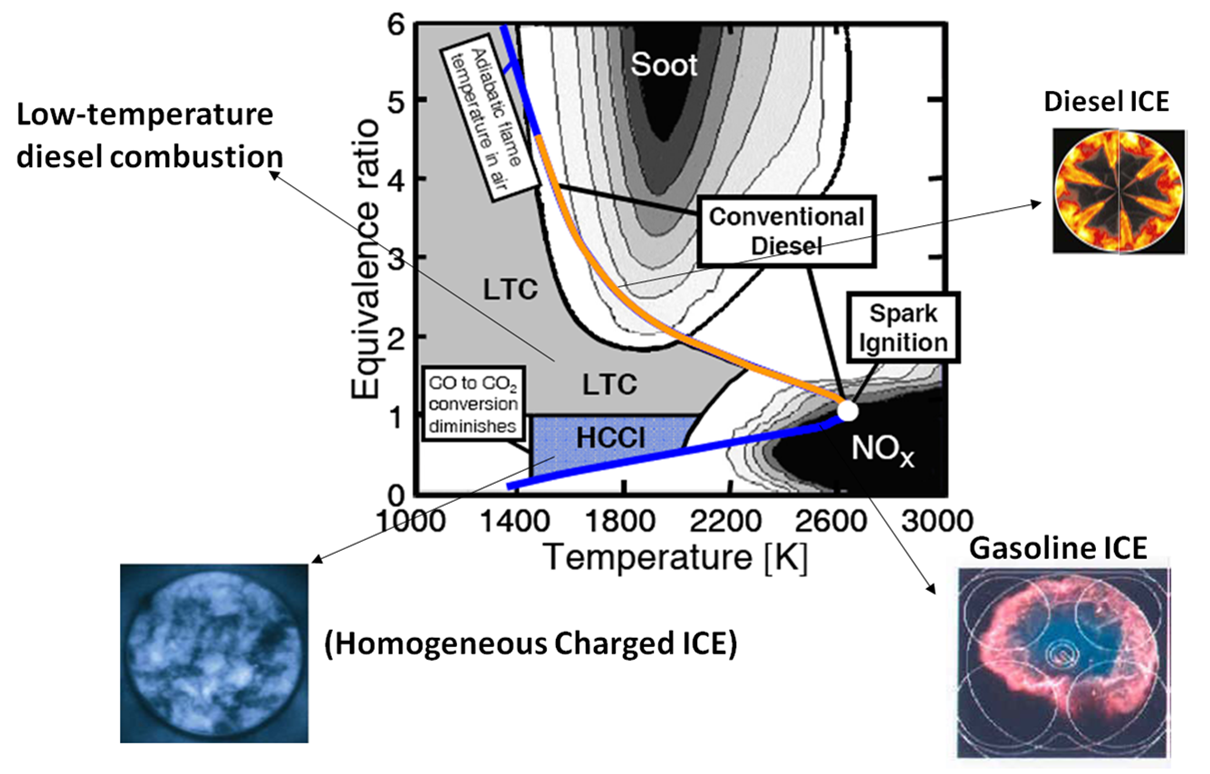
\includegraphics[width=\textwidth]{jackie-dec-engine}\\
        Reproduced in part from J.E. Dec, Proc. Combust. Inst. 32 (2009) 2727--2742
    \end{center}
\end{frame}

\againframe<5>{economy}

\begin{frame}<1>[label=betterfuels]{Better fuels have lower emissions and reduce dependence on fossil fuels}
    \setbeamercovered{transparent=15}
    \begin{itemize}
        \item<+- | uncover@+> Better fuels help move us away from traditional fuel sources
        \item<visible@+ | uncover@+> Better fuels help reduce total emissions
    \end{itemize}
\end{frame}

\begin{frame}{Methylcyclohexane is a major component in stepping-stone fuels}
    \begin{itemize}
        \item Methylcyclohexane (MCH) is an important component of fuels
            produced from alternative petroleum sources, such as shale oil
        \item Models of real transportation fuels are difficult to
            construct and use due to the chemical complexity of the fuels
        \item Surrogate models use a limited number of components to
            represent the chemical and physical properties of the real fuel
        \item MCH is a component in many surrogate transportation fuel
            formulations
    \end{itemize}
\end{frame}

\againframe<2>{betterfuels}

\begin{frame}{Bio-alcohol fuels can be sustainably produced to reduce well-to-wheel emissions}
    \begin{columns}
        \column{0.5\textwidth}
            \begin{itemize}
                \item Ethanol is a very common biofuel in use today
                \item Alcohols with more carbon atoms have higher energy density
                \item Butanol and pentanol can be produced from bio-based and waste sources
                \item Butanol is the smallest alcohol with each type of C-O bond
            \end{itemize}
        \column{0.5\textwidth}
            \centering
            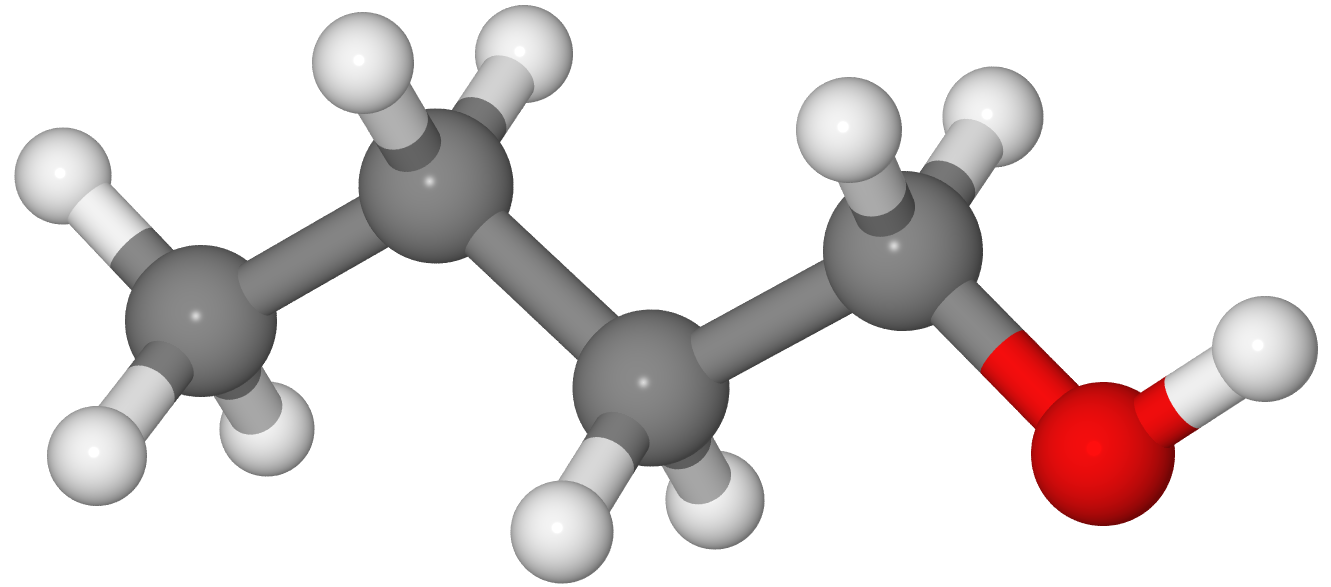
\includegraphics[height=0.18\textheight]{1-butanol}\par
            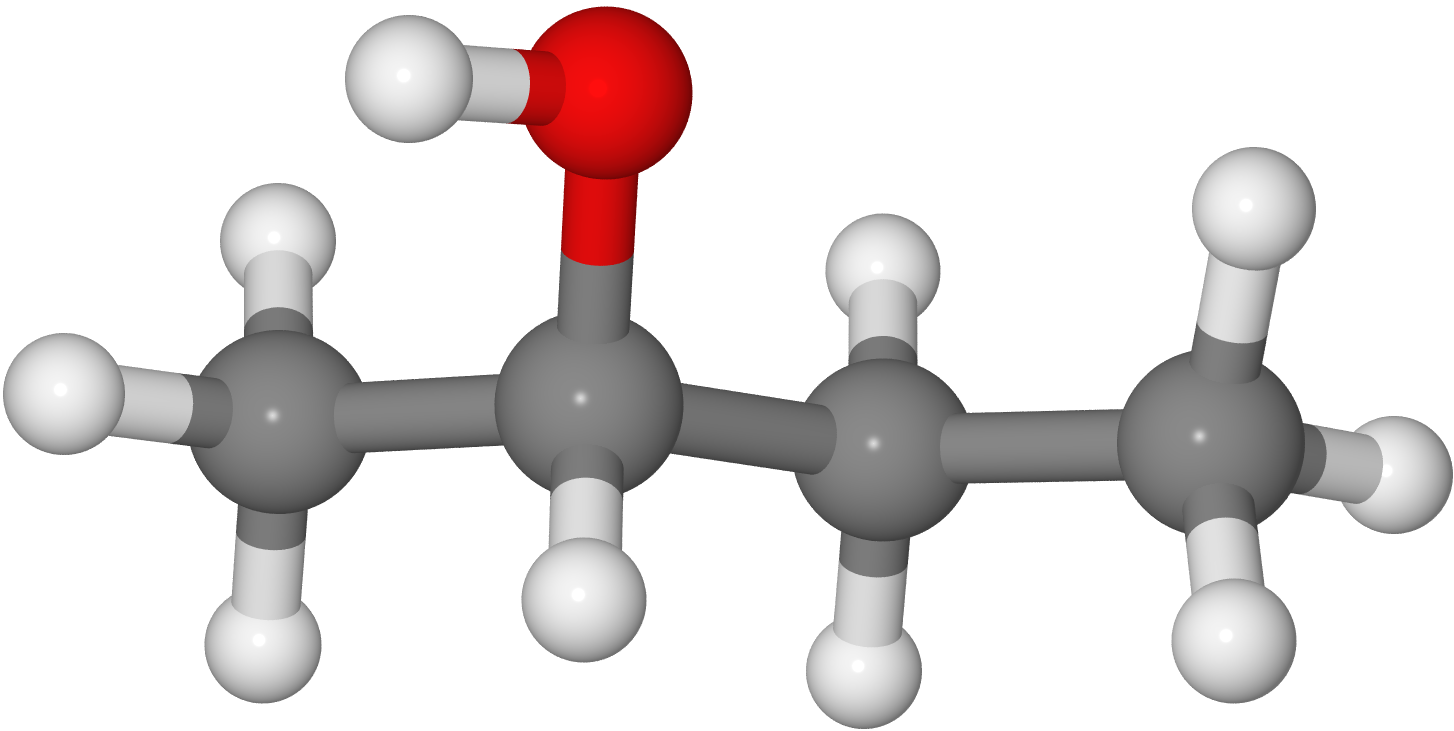
\includegraphics[height=0.18\textheight]{2-butanol}\par
            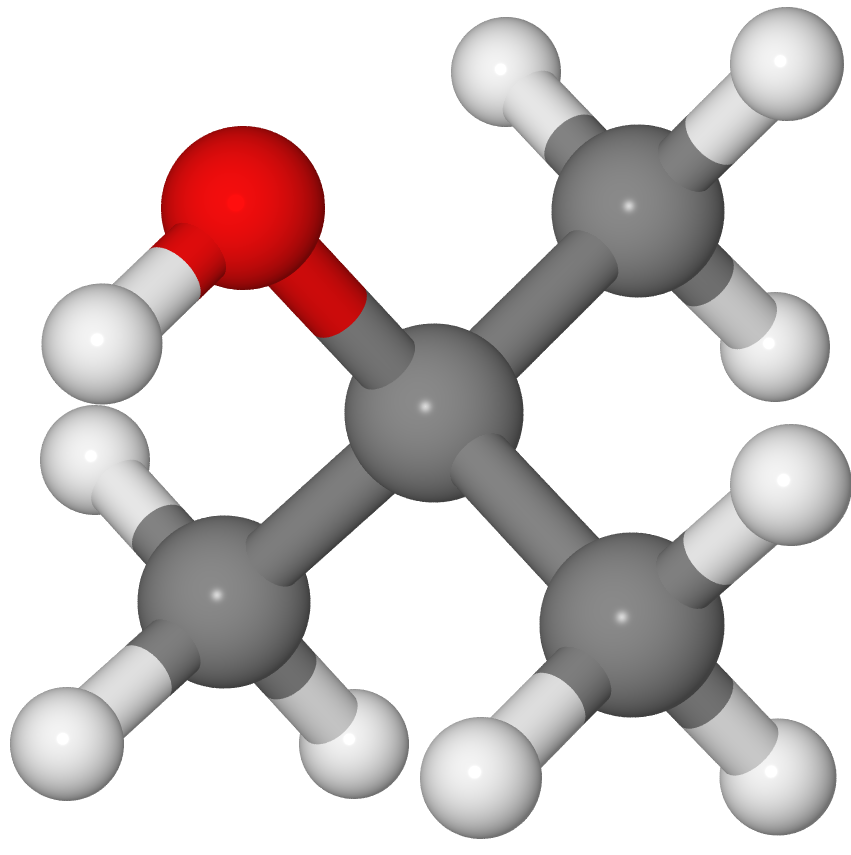
\includegraphics[height=0.18\textheight]{t-butanol}\par
            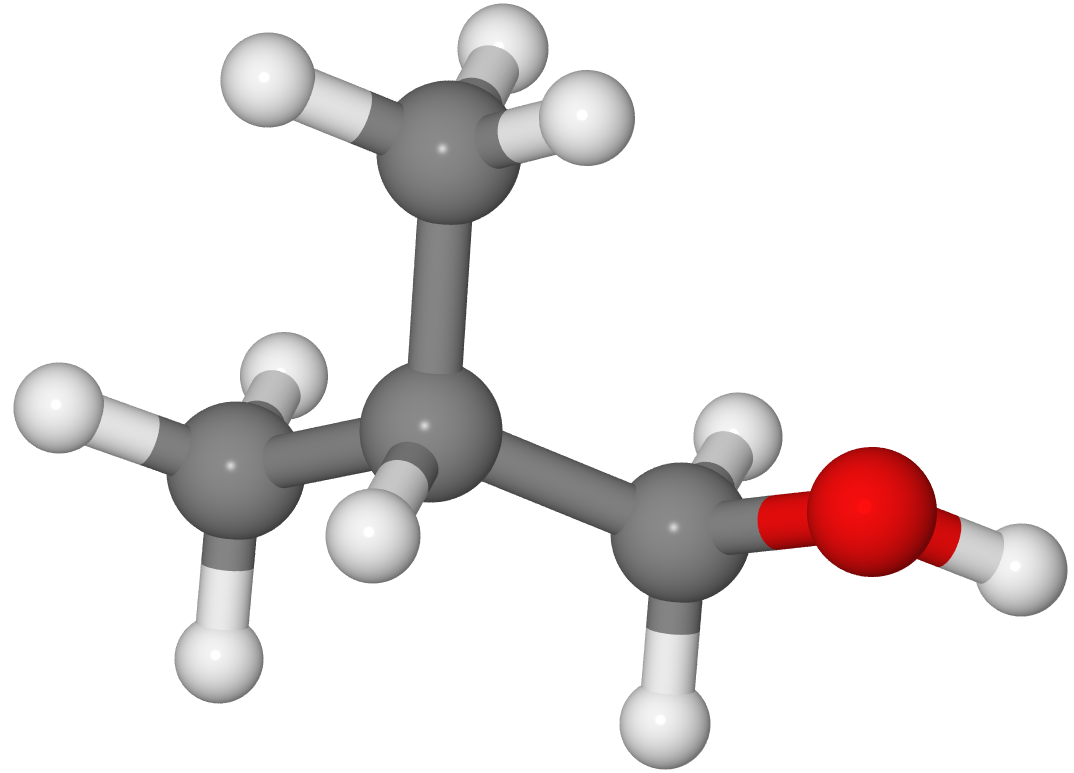
\includegraphics[height=0.18\textheight]{iso-butanol}\par
            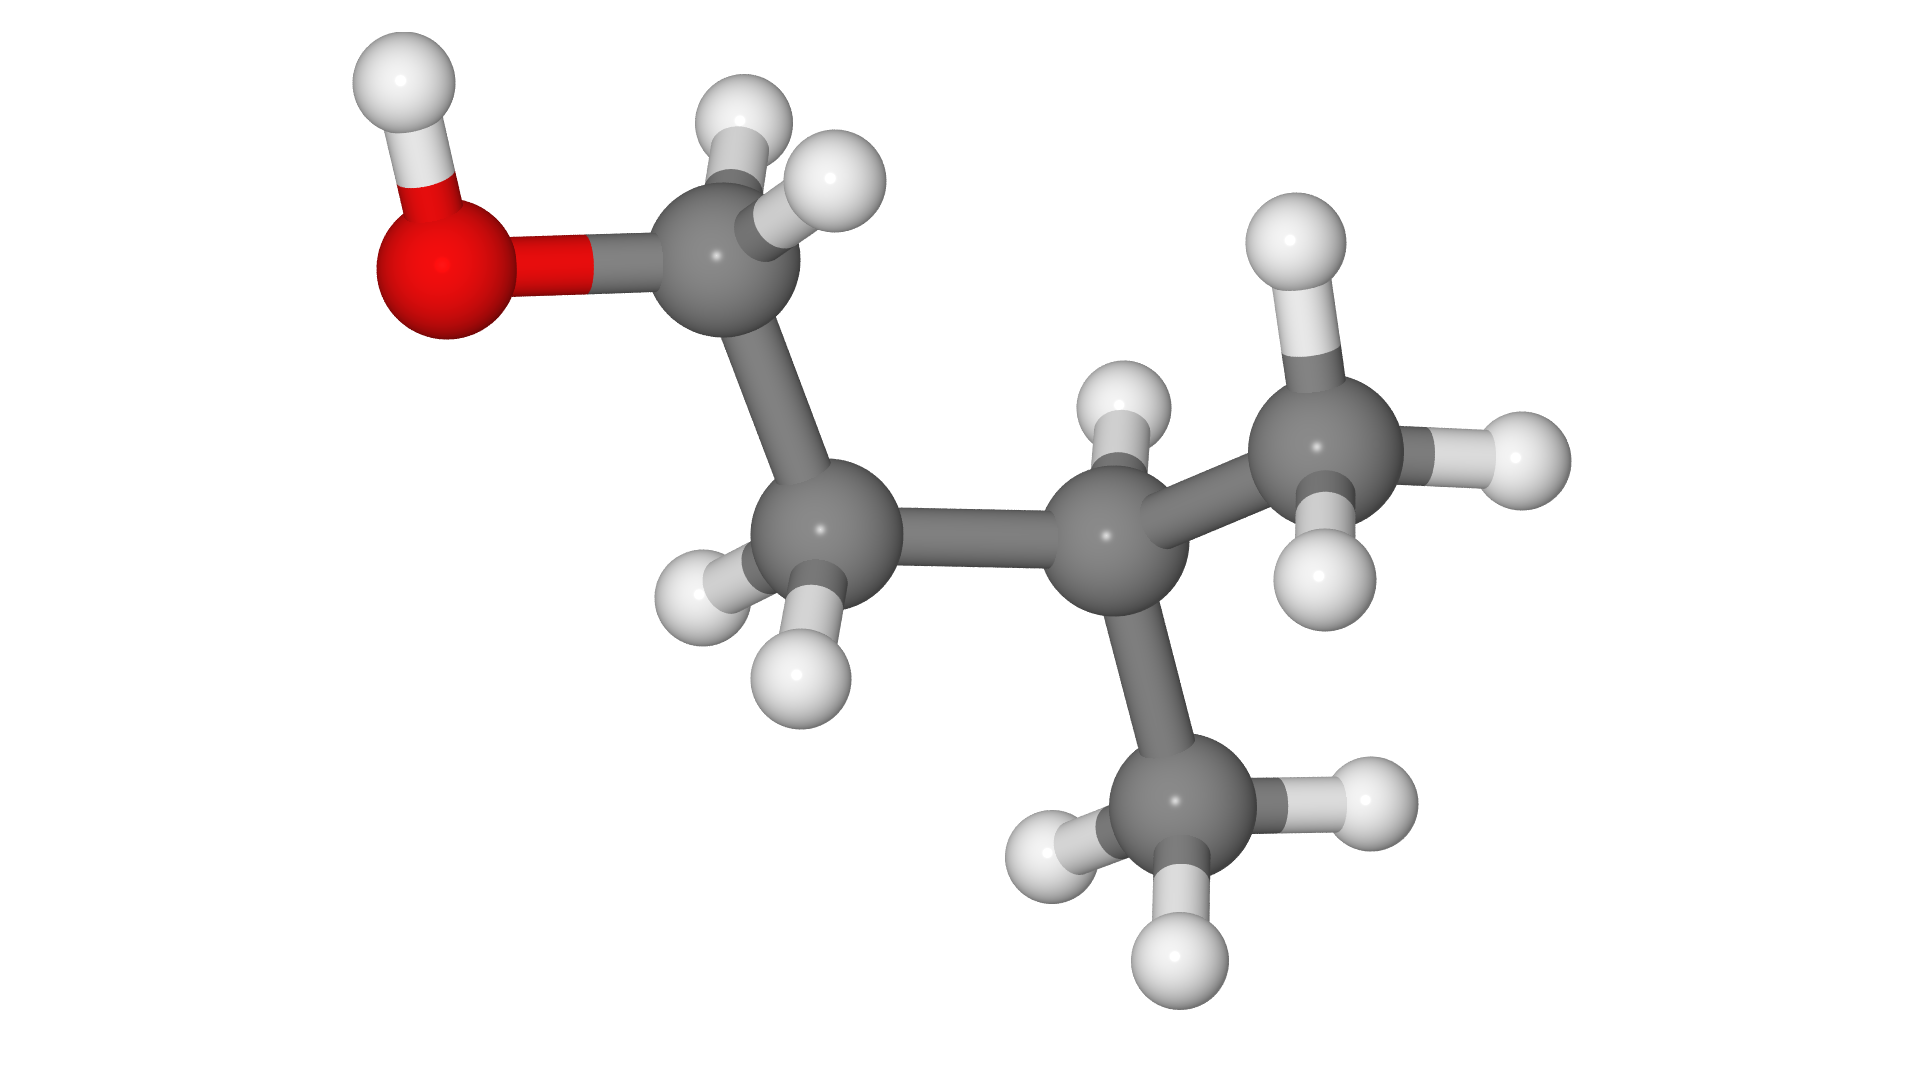
\includegraphics[height=0.18\textheight]{ipentanol}
    \end{columns}
\end{frame}

\begin{frame}{We need both solutions to make substantial progress}
    \begin{columns}
        \column{0.5\textwidth}
            \begin{itemize}
                \item<+-> Selecting the ``best'' alternative fuel requires knowledge
                    of the ``best'' engine, which depends on which
                    alternative fuel is selected\ldots
                \item<.-> Testing every fuel in every engine is prohibitively expensive
                    and time consuming
                \item<+-> Computer-aided design can be employed to create fuel-flexible
                    engines \alert{if the fuel models are predictive under LTC conditions}
            \end{itemize}
        \column{0.5\textwidth}
            \centering
            \only<2>{\setbeamercovered{transparent=15}}
            \begin{tikzpicture}[scale=0.6]
                \uncover<1>{\fill[even odd rule,red!30] circle (3.8) circle (3.2);
                \arcarrow{3}{3.5}{4}{-80}{80}{5}{blue,draw=red!50!black,very thick}{Best Advanced Engine}{white}
                \arcarrow{3}{3.5}{4}{100}{260}{5}{blue,draw=red!50!black,very thick}{Best Alternative Fuel}{white}}
                \node<2> at (0,0) {
\includegraphics[width=0.87\textwidth]{computer}};
            \end{tikzpicture}
    \end{columns}
\end{frame}

\begin{frame}
    \begin{center}
    \begin{tikzpicture}
    \begin{semilogyaxis}[
        table/col sep=comma,
        ylabel style={align=center,yshift=-5pt},
        xlabel style={align=center,yshift=5},
        ylabel={Reactivity\\$\leftarrow$Higher\qquad\qquad Lower$\rightarrow$},
        xlabel={$\leftarrow$Higher\qquad\qquad Lower$\rightarrow$\\Temperature},
        yticklabels={,,},
        xticklabels={,,},
        xmin=0.7,xmax=1.5,
        ymin=0.02,ymax=200,
        tick style = {color=black, semithick},
        minor tick style={thin},
        axis line style={semithick},
        every axis plot/.append style={%
            semithick,
        },
        every axis legend/.append style={
            legend pos=south east,
            anchor=south east,
            font=\tiny,
        },
        legend columns=1,
    ]
    \only<1-6>{\addplot[only marks,mark=square*,red] table[x=Hi-T-Real-Tc, y=Hi-T-Real-Ign] {figures/alcohol-models/model-data.csv};
    \addlegendentry{High Temperature Alkane}}
    \only<2-6>{\addplot[no markers,cyan] table[x=Hi-T-Alc-Tc, y expr=\thisrow{Hi-T-Alc-Mod}*0.75] {figures/alcohol-models/model-data.csv};
    \addlegendentry{High Temperature Model}}
    \only<3-6>{\addplot[only marks,mark=diamond*,black] table[x=Lo-T-Real-Tc, y=Lo-T-Real-Ign] {figures/alcohol-models/model-data.csv};
    \addlegendentry{Low Temperature Alkane}}
    \only<4-6>{\addplot[no markers,orange] table[x=Real-Mod-Tc, y=Real-Mod-Ign] {figures/alcohol-models/model-data.csv};
    \addlegendentry{Comprehensive Alkane Model}}
    \only<5->{\addplot[mark=*,blue,only marks,restrict x to domain=0.7:1.15] table[x=Alcohol-Tc, y=Alcohol-Ign] {figures/alcohol-models/model-data.csv};
    \addlegendentry{High Temperature Alcohol}}
    \only<6->{\addplot[only marks,mark=oplus*,violet,restrict x to domain=1.15:1.5] table[x=Alcohol-Tc, y=Alcohol-Ign] {figures/alcohol-models/model-data.csv};
    \addlegendentry{Low Temperature Alcohol}}
    \only<7>{\addplot[no markers,green!40!black,] table[x={1000/T_(1/K)},y expr=1000*\thisrow{Ignition time 3 by max dT/dt_(sec)}] {figures/alcohol-models/export.csv};
    \addlegendentry{Alcohol by Analogy to Alkane}}
    \only<8->{\addplot[no markers,domain=0.8:1.4,gray] {1.4097*x^12.714};
    \addlegendentry{Comprehensive Alcohol Model}}
    \end{semilogyaxis}
    \end{tikzpicture}
    \end{center}
\end{frame}

\end{document}
